\documentclass[tikz,border=1mm]{standalone}
\usepackage[T1]{fontenc}
\usepackage[swedish,english]{babel}
\usepackage{amsmath}
\usepackage{tikz}
\usepackage{amssymb}
\usetikzlibrary{shadows}
\usetikzlibrary{arrows,positioning}
\usepackage{pgfplots}
\begin{document}
% THE PICTURE BEGINS HEY?!!!
\begin{tikzpicture}[scale=1]
\definecolor{myBlue}{RGB}{57,106,177}; % (r,g,b) = (57,106,177)
\definecolor{myBrown}{RGB}{148,139,61};% (r,g,b) = (148,139,61)
% ORANGE HEY?
\definecolor{myOrange}{RGB}{213,94,0}
\definecolor{myBlueish}{RGB}{0,158,115}
%-----------------------------------------------------------------------------------------------------------------------------
% UPPER ROW
%-----------------------------------------------------------------------------------------------------------------------------
% Classic
\node at (-9,0) (A){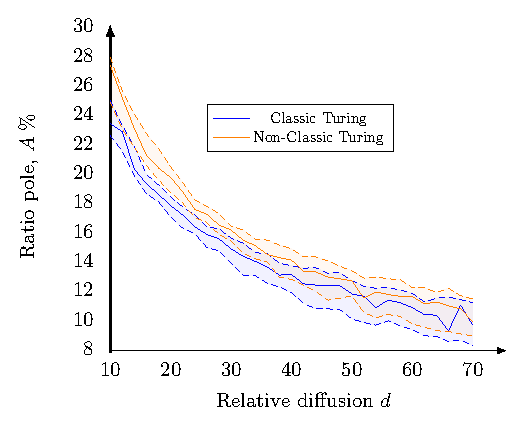
\includegraphics[scale=1.0]{./ratioPole/ratioPole.pdf}};
\node at (0,0) (B){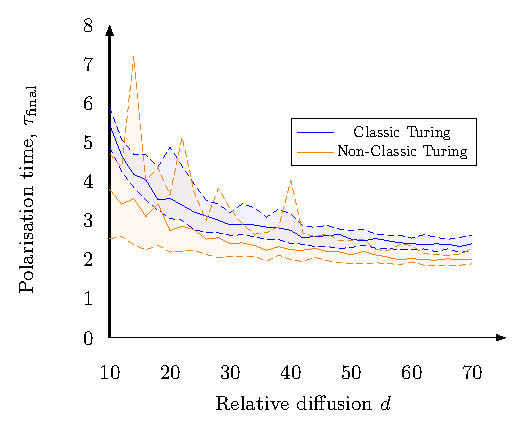
\includegraphics[scale=1.0]{./polTime/polTime.pdf}};
\node at (9,0) (C){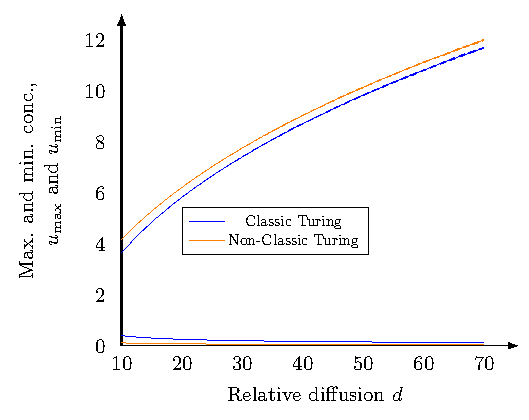
\includegraphics[scale=1.0]{./maxMin/maxMin.pdf}};
%-----------------------------------------------------------------------------------------------------------------------------
% LABELS OF THE VARIOUS SUB-FIGURES
%----------------------------------------------------------------------------------------------------------------------------- 
% Classic
%\node at (-14,5.0)(C) {\huge\textbf{(A)}};
\node at (-11.75,4.5)(C) {\Large \textbf{(A)}};
\node at (-2.75,4.5)(C) {\Large \textbf{(B)}};
\node at (6.25,4.5)(C) {\Large \textbf{(C)}};
%-----------------------------------------------------------------------------------------------------------------------------
%-----------------------------------------------------------------------------------------------------------------------------
\end{tikzpicture}
%-----------------------------------------------------------------------------------------------------------------------------
%-----------------------------------------------------------------------------------------------------------------------------
\end{document}
